\documentclass[11pt]{article}
\usepackage[margin=1in]{geometry}
\usepackage[T1]{fontenc}
\usepackage{lmodern}
\usepackage{microtype}
\usepackage{booktabs}
\usepackage{tabularx}
\usepackage{array}
\usepackage{enumitem}
\usepackage{xcolor}
\usepackage[normalem]{ulem}
\usepackage{tikz}
\usetikzlibrary{positioning,arrows.meta}
\usepackage[hidelinks]{hyperref}

\setlist{nosep,leftmargin=*}
\setlength{\parindent}{0pt}
\setlength{\parskip}{6pt}
\newcommand{\code}[1]{\texttt{#1}}
\newcolumntype{L}{>{\raggedright\arraybackslash}X}

\title{Open-Ended Multi-Agent Synthesis: Plan}
\author{22 September 2026}
\date{}

\begin{document}
\maketitle
\vspace{-1.5em}

This builds on \code{HANDOFF\_2026-09-06.md}, which remains correct for
everything not covered here. Every result below ran on cached generations, with
no API spend.

%-------------------------------------------------------------------
\section{What we want}

\textbf{Claim.} How an agent produced its answer carries evidence about each
claim's reliability, and that evidence does not depend on which agents are in
the pool. A synthesizer built on it can \textbf{swap the agents with no
relabelling}.

\textbf{System (v1).} Figure~\ref{fig:pipeline}. An LLM splits each response
into canonical claims; claims are matched across agents by exact string match on
their canonical form; a pool-invariant scorer turns the resulting claim table
into a probability per claim; a per-question budget splits claims into keep,
uncertain and drop; an LLM composer rules on the uncertain band, settles
contradictions and writes the answer.

\begin{figure}[p]
\centering
% Full process map of the synthesizer (v1). \input by PLAN_2026-09-22.tex and
% PIPELINE_2026-09-22.tex. Needs: tikz with positioning, arrows.meta.
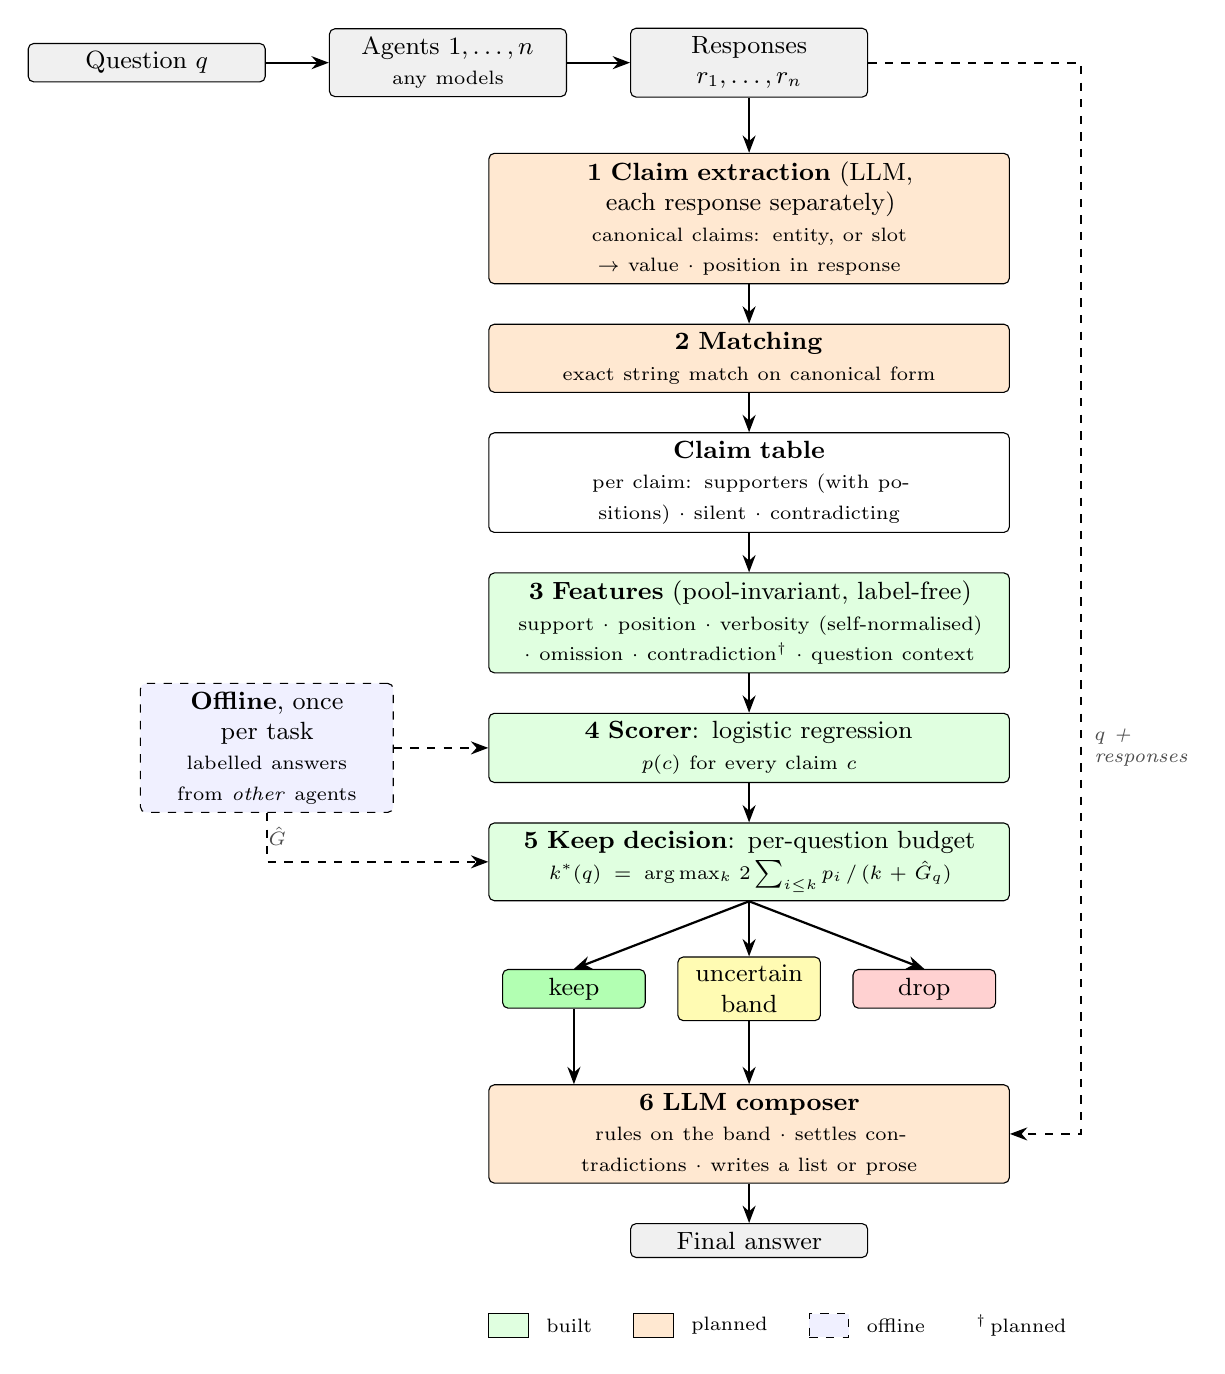
\begin{tikzpicture}[
  node distance=5mm and 8mm,
  >={Stealth[length=2.2mm]},
  box/.style={draw, rounded corners=2pt, align=center, text width=64mm,
              inner sep=3pt, font=\small},
  built/.style={box, fill=green!12},
  planned/.style={box, fill=orange!18},
  plain/.style={box, fill=white},
  io/.style={draw, rounded corners=2pt, align=center, text width=28mm,
             inner sep=3pt, font=\small, fill=gray!12},
  small/.style={draw, rounded corners=2pt, align=center, text width=16mm,
                inner sep=3pt, font=\small},
  offline/.style={draw, dashed, rounded corners=2pt, align=center,
                  text width=30mm, inner sep=3pt, font=\small, fill=blue!6},
  lab/.style={font=\scriptsize\itshape, text=black!70},
  flow/.style={->, thick},
  side/.style={->, thick, dashed},
]

% ---- inputs
\node[io] (resp) {Responses\\$r_1,\dots,r_n$};
\node[io, left=of resp] (agents) {Agents $1,\dots,n$\\{\scriptsize any models}};
\node[io, left=of agents] (q) {Question $q$};
\draw[flow] (q) -- (agents);
\draw[flow] (agents) -- (resp);

% ---- main column
\node[planned, below=7mm of resp] (extract)
  {\textbf{1~Claim extraction} (LLM, each response separately)\\
   {\scriptsize canonical claims: entity, or slot $\to$ value $\cdot$ position in response}};
\node[planned, below=of extract] (match)
  {\textbf{2~Matching}\\{\scriptsize exact string match on canonical form}};
\node[plain, below=of match] (table)
  {\textbf{Claim table}\\
   {\scriptsize per claim: supporters (with positions) $\cdot$ silent $\cdot$ contradicting}};
\node[built, below=of table] (feat)
  {\textbf{3~Features} (pool-invariant, label-free)\\
   {\scriptsize support $\cdot$ position $\cdot$ verbosity (self-normalised) $\cdot$
    omission $\cdot$ contradiction$^{\dagger}$ $\cdot$ question context}};
\node[built, below=of feat] (scorer)
  {\textbf{4~Scorer}: logistic regression\\{\scriptsize $p(c)$ for every claim $c$}};
\node[built, below=of scorer] (keep)
  {\textbf{5~Keep decision}: per-question budget\\
   {\scriptsize $k^*(q)=\arg\max_k \,2\sum_{i\le k}p_i \,/\, (k+\hat G_q)$}};

% ---- three-way split
\node[small, fill=yellow!30, below=7mm of keep] (band) {uncertain\\band};
\node[small, fill=green!30, left=4mm of band] (hi) {keep};
\node[small, fill=red!18, right=4mm of band] (lo) {drop};
\draw[flow] (keep.south) -- (hi.north);
\draw[flow] (keep.south) -- (band.north);
\draw[flow] (keep.south) -- (lo.north);

% ---- composer and output
\node[planned, below=8mm of band] (comp)
  {\textbf{6~LLM composer}\\
   {\scriptsize rules on the band $\cdot$ settles contradictions $\cdot$
    writes a list or prose}};
\node[io, below=of comp] (ans) {Final answer};

% ---- main flow
\draw[flow] (resp) -- (extract);
\draw[flow] (extract) -- (match);
\draw[flow] (match) -- (table);
\draw[flow] (table) -- (feat);
\draw[flow] (feat) -- (scorer);
\draw[flow] (scorer) -- (keep);
\draw[flow] (hi.south) -- (hi.south |- comp.north);
\draw[flow] (band) -- (comp);
\draw[flow] (comp) -- (ans);

% ---- the composer also reads the question and the original responses
\coordinate (R) at ([xshift=9mm]feat.east);
\draw[side] (resp.east) -- (resp.east -| R) -- (comp.east -| R) -- (comp.east);
\node[lab, right=0.5mm, align=left] at (scorer.east -| R) {$q$ +\\responses};

% ---- offline training, once per task
\node[offline, left=12mm of scorer] (train)
  {\textbf{Offline}, once per task\\{\scriptsize labelled answers from \emph{other} agents}};
\draw[side] (train.east) -- (scorer.west);
\draw[side] (train.south) |- (keep.west);
\node[lab, below right=0.5mm and -1mm of train.south] {$\hat G$};

% ---- legend
\node[draw, fill=green!12, minimum width=5mm, minimum height=3mm, inner sep=0pt,
      below=7mm of ans.south west, anchor=north west, xshift=-18mm] (l1) {};
\node[right=1mm of l1, font=\scriptsize] (t1) {built};
\node[draw, fill=orange!18, minimum width=5mm, minimum height=3mm, inner sep=0pt,
      right=4mm of t1] (l2) {};
\node[right=1mm of l2, font=\scriptsize] (t2) {planned};
\node[draw, dashed, fill=blue!6, minimum width=5mm, minimum height=3mm, inner sep=0pt,
      right=4mm of t2] (l3) {};
\node[right=1mm of l3, font=\scriptsize] (t3) {offline};
\node[right=4mm of t3, font=\scriptsize] {$^{\dagger}$\,planned};
\end{tikzpicture}

\caption{The v1 process, one question at a time. Steps 1--2 build a claim table
for any answer format; steps 3--5 are the scorer trained once per task on
labelled answers from other agents, so new agents need no labels; step 6 is the
only step that writes text. The composer also receives the question and the
original responses (dashed, right). $\hat G$ is the predicted gold count used
by the budget.}
\label{fig:pipeline}
\end{figure}

\textbf{Zero-label: decided 22 September.} Zero-label means \emph{no labels
for the new agent pool}. Labelled data from the same task with other agents may
train the scorer.
\begin{itemize}
  \item \textbf{New pool, known task:} supported strongly (\S\ref{sec:findings}).
        This is the realistic multi-agent case: models change every month, the
        task does not.
  \item \textbf{New task:} a stress test with a stated boundary, not a
        requirement. On list-F1 benchmarks the scorer's value is mostly deciding
        how many answers to keep, and that is fixed by how each dataset built its
        gold. WebQSP's Freebase gold averages 76 answers per question; QAMPARI's
        gold is incomplete. Test cross-task only with a metric that does not
        depend on gold construction (judged claim precision plus recall against
        gold).
\end{itemize}

\textbf{Where the LLM must earn its place:} long-form composition, and judging
the uncertain claims. On lists the scorer alone may already be the best system.
The pilot decides (\S\ref{sec:pilot}).

%-------------------------------------------------------------------
\section{Findings}\label{sec:findings}

Code: \code{analysis/pool\_transfer.py}, \code{analysis/cut\_rules.py},
\code{analysis/position\_signal.py}. Results in \code{results/*.json} and the
matching \code{*.log} files.

\subsection{Pool transfer works, and the identity gap is closed without labels}

The scorer uses about 12 pool-invariant features plus \emph{self}
normalisation: rank and verbosity are measured against each agent's own median
list length. No labels are needed for any of it.

\begin{center}
\begin{tabularx}{\linewidth}{Lcc}
\toprule
QAMPARI, disjoint pools, question-disjoint & F1 & vs zero-label count \\
\midrule
4 $\to$ other 4 (70 transfers) & \textbf{27.63} & \textbf{+4.91}, significant 70/70 \\
3 $\to$ other 5 (56) & 28.14 & +4.57, significant 46/56 (1 loss) \\
5 $\to$ other 3 (56) & 26.29 & +6.46, significant 56/56 \\
\midrule
Paper scorer, identity features, \emph{target gold}, 4-agent pools & 28.25 & --- \\
\bottomrule
\end{tabularx}
\end{center}

\begin{itemize}
  \item The transferred scorer beats counting even when counting's threshold is
        tuned on target gold (23.94, 4-agent pools).
  \item It comes within 0.4--1.2 F1 of the fully supervised paper scorer.
  \item \textbf{Runway:} the gain does not shrink as the pool's best agent gets
        stronger (correlation $+0.02$ across 70 pools). This differs from
        MAS-Orchestra, though our best-single range is narrow (24--28).
\end{itemize}

\subsection{Dead ends, measured}
\begin{itemize}
  \item Reliability features (agreement, Dawid--Skene, supervised) break transfer.
  \item Prior-shift recalibration: the estimated base rate collapses.
  \item Multi-source training does not help cross-task.
  \item ``Size from counting, content from scorer'' loses to counting at matched size.
\end{itemize}

\subsection{The scorer's value is per-question sizing, not reordering}

At the same output size as counting, the scorer is no better than counting
($-0.2$ to $-0.6$). Its gain comes from choosing \emph{how many} claims to keep
per question. That is why it transfers across pools, which share a gold
convention, but across tasks only where the conventions match:
\begin{itemize}
  \item CWQ: $+0.9$ to $+1.8$ from every source.
  \item WebQSP: $-0.6$ to $-3.4$.
  \item QAMPARI, from the knowledge-graph datasets: $-0.4$ to $-3.6$.
\end{itemize}

\subsection{Position is real but modest; it stays in the scorer}

\textbf{Real.} With support and list length controlled, per (claim, agent),
later items are less often correct on all three datasets.

\begin{center}
\begin{tabular}{lcc}
\toprule
Solo claims, 6--100 item lists & Top depth quintile & Bottom depth quintile \\
\midrule
QAMPARI & 5.6\% & 1.8\% \\
CWQ     & 7.2\% & 4.2\% \\
WebQSP  & 11.8\% & 7.4\% \\
\bottomrule
\end{tabular}
\end{center}

Shared claims show the same pattern (QAMPARI 36\% $\to$ 20\%, WebQSP 61\%
$\to$ 39\%). The effect survives on WebQSP's near-exhaustive gold, so it is
not only a ``famous entities are in the gold list'' artefact; QAMPARI's
steeper gradient may partly be one. It reverses on 1--5 item lists.

\textbf{Decomposition} of the $+4.91$ gain over counting (zero-label 4\,$|$\,4
transfer):

\begin{center}
\begin{tabular}{lc}
\toprule
Component & F1 over counting \\
\midrule
Per-question budget on support alone & +2.67 \\
Question context (number of candidates, mean support) & +0.78 \\
Rank + verbosity + omission together & +1.46 \\
\bottomrule
\end{tabular}
\end{center}

\begin{itemize}
  \item Dropped one at a time: rank $-0.51$, verbosity $-0.42$, omission $-0.01$.
  \item Pool-invariant omission adds nothing. Its earlier $+1.65$ came from
        knowing \emph{which} agent was silent, which is identity.
  \item \textbf{Decided:} position stays in the scorer. Removing it is
        significantly worse in 40/70 splits, it needs no labels, and its
        direction is the same on all three datasets. The change is in framing,
        not features.
  \item \textbf{Framing:} the headline mechanism is sizing each answer from the
        crowd's agreement structure. Per-claim behavioural signals are a real but
        secondary $+1.5$. Generated-position confidence also has prior art
        (\code{NOVELTY\_CHECK.md}).
\end{itemize}

\subsection{Long-form: sentence clustering merges contradictions}
\begin{itemize}
  \item Hand-check marked 22 September (\code{docs/ASQA\_MATCHING\_HANDCHECK.md},
        rule and per-item reasons in the file). Only 12/20 groups state one
        fact; 5/20 merge \emph{contradicting values} (A17: 91.5 vs 47.5 sacks;
        A19: 41 vs 43 parks; A4: 2019 vs 2020; A13; A3), and 3 bundle
        different facts.
  \item Of 20 near-miss pairs below the threshold, 7 are missed matches and
        3--4 are same-slot contradictions (B7, B9, B16).
  \item 87\% of clusters are single-agent.
  \item Sentence similarity cannot tell agreement from contradiction, so
        contradicting agents are counted as support.
\end{itemize}

\subsection{Gold is very incomplete}
Union precision is 4--11\% on all three list datasets. Any arm that adds
correct but unlisted items, such as the LLM or \code{solo} arms, is penalised.

%-------------------------------------------------------------------
\section{Design decisions}
\begin{enumerate}
  \item \textbf{Scorer:} pool-invariant and self-normalised, with position and
        verbosity features kept and no reliability block. The paper scorer
        becomes an in-pool supervised reference.
  \item \textbf{One claim splitter for every format: LLM canonical extraction.}
        An LLM reads each response \emph{separately} and rewrites every claim in
        canonical form: full official entity names (``MGM'' $\to$
        ``Metro-Goldwyn-Mayer''), numbers as plain values, and for prose a
        slot $\to$ value pair with consistently phrased slots. Matching across
        agents is then exact string comparison, so the LLM never judges whether
        two different claims are the same. This replaces the regex list parser
        and the sentence-embedding clustering.
        \begin{itemize}
          \item \emph{Why not LLM clustering:} the 18 August attempt merged
                claims across agents and made false merges (``Yale Law School''
                with ``University of Michigan Law School''), and it kept one
                representative per cluster, so a false merge deleted a correct
                answer. Per-response canonicalisation has no merge step.
          \item \emph{Its failure mode is inconsistency:} two calls may
                canonicalise one entity differently. That is a missed match,
                which lowers a support count, not a false merge, which deletes
                an answer.
          \item \emph{Contradiction:} values in the same slot compete, so a
                \emph{contradicting} agent is distinct from a \emph{silent} one.
                Lists never had this signal. All scorer features port.
        \end{itemize}
  \item \textbf{Long-form position:} keep sentence position as a feature, but
        ablate it with and without before trusting it. First sentences are often
        hedges.
  \item \textbf{Long-form metric:} judged fact precision $\times$ STR-EM recall
        over ASQA's interpretations. DR is length-dominated, which would make
        length a gold-convention choice again.
  \item \textbf{Composer = band:} the scorer decides confident claims; the LLM
        rules on the uncertain band and writes the answer. Answer-count
        estimation by an LLM is capped at about 1--2 F1 (true-count oracle), so
        it is not the LLM's job.
  \item \textbf{Every LLM result is reported with its output size} and against
        the no-LLM \code{scorer} reference.
\end{enumerate}

%-------------------------------------------------------------------
\section{Pilot: what each outcome means (written before running)}\label{sec:pilot}

Arms: \code{text}, \code{evidence}, \code{scramble}, \code{p},
\code{pscramble}, \code{solo}, plus the no-LLM \code{scorer} reference.

\begin{center}
\small
\begin{tabularx}{\linewidth}{LLL}
\toprule
Outcome & Meaning & Next \\
\midrule
\code{p} $>$ \code{text}, \code{p} $-$ \code{pscramble} $>0$, \code{p} $\ge$ \code{scorer}
  & Evidence-augmented synthesis works & Centre the paper on it \\
\code{p} $\approx$ \code{pscramble} & The LLM ignores the numbers & Band composer, hard-gated \\
\code{scorer} $\ge$ every LLM arm & Lists don't need an LLM & LLM only for long-form composition \\
\code{solo} $\approx$ \code{text} or better & Synthesizer's own knowledge dominates & Weaker synthesizer, or report relative to \code{solo} \\
An arm wins but lists far more or fewer items & Size effect, not synthesis & Compare at matched size \\
\bottomrule
\end{tabularx}
\end{center}

%-------------------------------------------------------------------
\section{v2: internal model signals (after v1's baseline comparisons)}

Added 22 September. Only if the scorer has room to improve. Each step is
measured the same way as position: F1 with and without, in the zero-label pool
transfer.

\begin{center}
\small
\begin{tabularx}{\linewidth}{cLLLl}
\toprule
Step & Signal & Access & Zero-label? & Decision \\
\midrule
1 & \textbf{Per-claim token log-probabilities}: the model's confidence while
    writing each claim
  & Many APIs return them (OpenAI, some Azure deployments)
  & Yes, if normalised against each agent's own typical values, as for verbosity
  & \textbf{Do after v1} \\
2 & Hidden-state probes & Open-weight models only
  & Only with unsupervised probes; a trained probe per new model needs that
    model's labels
  & Maybe, as an extension \\
3 & KV-cache or hidden-state sharing between agents
  & Open weights, usually one model family & ---
  & \textbf{Skip} \\
\bottomrule
\end{tabularx}
\end{center}

\begin{itemize}
  \item \textbf{Why step 1:} UAF uses perplexity-style signals but one number
        per response. Per-claim log-probabilities say \emph{which item} in a
        list the model was unsure about. It is a direct head-to-head with UAF,
        and it keeps the closed-model setting.
  \item \textbf{How it enters:} new scorer features, such as the supporters'
        mean self-normalised log-probability. Nothing else in the pipeline
        changes.
  \item \textbf{Why skip step 3:} it addresses agents reasoning together, not
        merging finished answers.
  \item \textbf{Cost:} re-query a sample with log-probabilities on. Check first
        which pool models expose them.
\end{itemize}

%-------------------------------------------------------------------
\section{Actions}

\begin{center}
\small
\begin{tabularx}{\linewidth}{cLl}
\toprule
\# & Action & Cost \\
\midrule
1 & \sout{Decide the zero-label definition}. Done: new pool, not new task. & --- \\
2 & \sout{Mark \code{docs/ASQA\_MATCHING\_HANDCHECK.md}}. Done 22 September. & --- \\
2a & Score the cached 18 August LLM merges against QAMPARI gold aliases
     (merge precision and recall). & CPU \\
2b & Canonical extraction on 100 QAMPARI questions; measure missed matches and
     false matches against gold aliases, and F1 against the regex parser. & $\sim$\$1 \\
3 & Top up OpenRouter and run the pilot (command below). & $\sim$\$1--4 \\
4 & Canonical slot$\to$value extraction on 50 ASQA questions; hand-check 20. & $\sim$\$1 \\
5 & ASQA features on slot$\to$value claims; test contradiction $\neq$ omission;
    ablate sentence position; ASQA pool transfer (3\,$\leftrightarrow$\,3 of 6 agents). & CPU \\
6 & Judge-audit 100 list outputs to measure gold incompleteness before reading the pilot. & $\sim$\$1 \\
7 & Band composer arm. & CPU, then $\sim$\$2 \\
\bottomrule
\end{tabularx}
\end{center}

Pilot command:
\begin{verbatim}
./venv/bin/python -u -m open_ended_aggregation.analysis.synth_rungs \
    --bench cwq --n 120 --synth openai/gpt-5.4
\end{verbatim}
About 1.0M input tokens. \code{--dry-run} checks the prompts for free. The
\code{p} arm uses the self-normalised scorer fitted on QAMPARI, so it is
zero-label on CWQ.

\textbf{ACL Findings ($\sim$Oct 10--12)} still needs the five stale floats, the
log-space $\hat G$ patch, WebQSP and ASC, all on CPU. The pool-transfer result
answers the paper's biggest weakness (a scorer parameterised by agent identity)
and is ready to add as a section. Decision pending.

%-------------------------------------------------------------------
\section{Files}
\begin{itemize}
  \item \textbf{Figure:} \code{pipeline\_tikz.tex} (the diagram, \verb|\input| by
        this plan) and \code{PIPELINE\_2026-09-22.tex} (standalone build).
  \item \textbf{New:} \code{analysis/pool\_transfer.py}, \code{analysis/cut\_rules.py},
        \code{analysis/position\_signal.py}; \code{results/pool\_transfer.json},
        \code{results/pool\_transfer\_part3.json}, \code{results/cut\_rules.json},
        \code{results/position\_signal.json}; the matching \code{.log} files;
        \code{docs/ASQA\_MATCHING\_HANDCHECK.md}.
  \item The 3\,$\leftrightarrow$\,5 pool-size numbers came from an inline run
        whose JSON write failed; they are recorded only in this plan.
  \item \textbf{Edited:} \code{analysis/synth\_rungs.py}: order randomisation;
        \code{p}, \code{pscramble} and \code{solo} arms; \code{scorer} reference;
        per-arm output size; \code{--dry-run}; verbatim-copy instruction. Each
        change was checked against a mock backend.
  \item Nothing committed; the tree already had uncommitted changes.
\end{itemize}

\end{document}
